\documentclass{article}
\usepackage[utf8]{inputenc}
\usepackage{graphicx}
\graphicspath{ {Images/} }

\title{AAMLP Project: Predicting Detailed Recidivism Outcomes}
\author{Eileen Patten}
\date{April 2018}

\begin{document}

\maketitle

\section{Abstract}

The Pennsylvania Commission on Sentencing has contracted Heinz College students to assess the feasibility of developing a more empirically based Prior Record Score to be used in sentencing. Sentencing guidelines in Pennsylvania have two components: the offense gravity score (OGS) that considers the severity of the current crime, and the prior record score (PRS), which is a measure of past criminal behavior that is used to lengthen sentences. While the primary focus of the systems project has been on building a new PRS around general recidivism risk, practical and policy considerations, stakeholders in the justice community have expressed a desire to know not just whether someone will recidivate, but whether they will commit any serious or violent crimes in the future. The aim of this analysis is to attempt to predict the offense grade of a future criminal event (i.e., misdemeanor or felony). Prediction of this more detailed recidivism is accomplished with an AUC similar to that for the general recidivism task, and shows promise as an added feature to the sentencing practice.

\section{Introduction and Background}
Sentencing guidelines in Pennsylvania have two components: the offense gravity score (OGS) that considers the severity of the current crime, and the prior record score (PRS), which is a measure of past criminal behavior that is used to lengthen sentences.\cite{code} The current Pennsylvania PRS considers the number and nature of prior criminal convictions and juvenile adjudications. For each judicial proceeding on one's record, the most serious offense is given points between 0 and 4, which are added up to compute a prior record score of 0 through 5, with a cap set at 3 for those who have only misdemeanor offenses. Offenders are then classified into PRS categories either based on their point score (0-5), or through placement into the special PRS eligibility categories RFEL (Repeat Felony 1 and Felony 2 Offender) or REVOC (Repeat Violent Offender). Below is an image showing the sentencing grid with recommended sentence lengths (in months). The OGS are the numbers 1 through 13 along the vertical axis and the PRS is along the horizontal axis:

\begin{center}
Figure 1: Pennsylvania's Sentencing Guidelines Grid
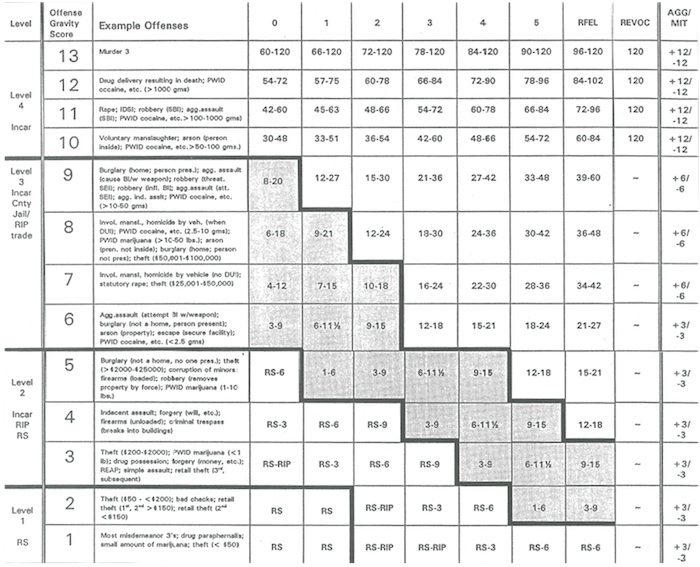
\includegraphics[scale=0.5]{sentencing_table.jpg}
\end{center}

The current scheme for arriving at an offender's PRS was developed in the late 1970s, with some adjustments over time. While utilitarian notions of public safety, risk, deterrence, and incapacitation appear to have been central to the policy discussion around the PRS, the PRS does not appear to have been empirically derived. Decisions about the PRS scoring system, the creation of the eight PRS categories, and the escalation in punishment for increasing PRS scores seem to have been based mostly on intuition and expertise, rather than empirical analysis aimed to identify and categorize offenders based on the likelihood of re-offending. 

The current project has aimed to construct one or more PRS alternatives that can serve to improve the sentencing process. Using data provided by our client, the Pennsylvania Commission on Sentencing, we are attempting to create alternatives to the PRS using recidivism risk as a primary determinant of the score and measure of empirical validity. At the same time, we are taking into consideration the views of different stakeholders, as well as the societal and demographic impacts of the current and proposed PRS.  

Much work has been done in creating actuarial recidivism risk models for the criminal justice system.\cite{review} The attempt to forecast risk goes back to the 1920s when various attempts were made to estimate the success of parole based on age, race, prior record, employment, schooling and neighborhood of residence (\cite{borden}, \cite{burgess}. More recently, machine learning techniques have been implemented in place of these more rudimentary methods. The hope, backed by research in the area, is that these actuarial methods will be better than clinical decision-making by judges at predicting recidivism risk, thus ensuring public safety is not compromised while at the same time effectively and efficiently utilizing public safety resources (\cite{dawes}, \cite{grove_and_meehl}).

But it should be made clear that the new PRS model this research is attempting to construct is not meant to be merely an actuarial risk model. For one thing, it should include only features of one's prior record, and not other details of one's demographics, personality, character, or medical history often included in such risk measures. For another, it must consider practical matters, such as forcing non-negative coefficients so that it does not appear that one, for example, could lower one's PRS category by committing certain types of crimes. Instead, only crime-free periods and an older age at first offense should act to lower a PRS score. Additionally, it is desirable for both deterrence and justice reasons that the model be interpretable to the point of being able to compute one's score on a simple calculator, so model type will be a key concern. Finally, it will maintain special categories for those with no (or only a very minor) prior record (PRS 0) and continue to place repeat felony and serious offenders in separate categories, regardless of their recidivism risk. These categories are instead to be understood as maintaining the dual purpose of retribution within the PRS model (or lack thereof for new offenders).

This effort is being carried out on behalf of the Pennsylvania Commission on Sentencing, which is currently undertaking a subcommittee review of the PRS. The analysis conducted by the team will inform this debate and suggest ways to improve the empirical validity of the PRS. 

At a midpoint presentation given to members of our advisory board, including judges, public defenders, and others in the justice community, there was broad support for some measure of not just whether an offender will recidivate, but how serious the re-offense will be. These professionals are focused on public safety, and are particularly concerned with protecting the public from violent or serious crime. While our main project continues to focus on a new model for the PRS based on general recidivism risk, this side analysis is attempting to address the desire for a prediction of a more detailed recidivism outcome. In this case, I will attempt to predict severity of future crimes by considering whether the first crime post-release will be a misdemeanor, felony, or whether there will be no recidivism event within the first 3 years following the start of community supervision or release from incarceration.

Many attempts have been made by other researchers to predict violent recidivism as opposed to general recidivism (for example, Prell et al. \cite{violence}) as well as specific types of violent recidivism (for example, Zeng et al. \cite{zeng}). However, to the best of my knowledge, no other attempts have been made to predict whether the rearrest will be for a misdemeanor or felony offense. Violent crimes are not the only serious crimes; crimes like burglary, identity theft, and arson can have serious impacts on society, even if they do not lead to physical harm of any person. This new approach will give the Commission another factor to consider in revising the PRS and giving more information to judges as they make their sentencing decisions.

\section{Methods}

\subsection{The Data}
In order to pursue this research, the Pennsylvania Commission on Sentencing (PCS) has provided the project team with a dataset consisting of approximately 131,000 offenders sentenced in Pennsylvania in 2004-2006 who were followed for three years upon the initiation of community supervision or release from incarceration to determine the occurrence of recidivism (n= 130,758). The data for this study were collected by the PCS as part of a separate project to develop an actuarial risk assessment tool for use in sentencing. Information on prison release dates, re-arrest, and technical violations of parole leading to recommitment were obtained through requests to the Pennsylvania Department of Corrections and the Pennsylvania State Police. Information on prior crimes were drawn from RAP sheets (i.e., criminal records) requested from the Pennsylvania State Police. 

This data includes every person sentenced during this time and released by July 2011, rather than a sample of offenders over this period, with a few exceptions noted below. 

Firstly, the data was collected only through July 2014, so includes offenders who were released as of July 2011. This means that many of the most serious offenders, with sentence lengths beyond 5-7 years, will not be included in our data. In total, 2,001 individuals were still in prison in July 2014 and 2,026 had not been out of jail or prison long enough to observe 3-year recidivism rates. The data also excludes life and death sentences (n=396) and cases with only DUI offenses (n=51,272). In this way, the study design might not generalize to the minority of offenders committing the most serious crimes, or to those committing only DUI offenses.

Additionally, the time period of this data straddles the Great Recession of 2007-09. While crime continued to fall during this recession, baffling many criminologists who expected crime to rise under a bad economy, it is still possible that the particular nature of the time in which our data was collected may impact the external validity of the findings.\cite{freak} We do, in fact, observe a spike in recidivism rates for offenders who were released in 2007, and spent the majority of their first 3 years following release in the economic recession.

Finally, the data does not capture scenarios where offenders recidivated outside the Commonwealth of Pennsylvania, as only Pennsylvania crimes are captured.

\subsection{Feature Selection}

While our data includes a large number of features, many of them are improper to use in our prediction task because they are forward-looking. We must only use features that would be known to a judge at the time of sentencing. Information on the prior record is limited to counts of prior offenses. Offenses were dropped if there were less than 50 instances of that prior offense in the data when it was observed that some of these crimes often received unduly large coefficients in the models. Categorical variables were also adjusted so that each level had a sufficient number of cases. 

The data is limited in that it includes no information on the timing of prior criminal events, except for the Age at First Arrest, and there is no information about time spent incarcerated or under community supervision, except for the present crime. Additionally, we had to drop all details about juvenile crimes from our data due to concerns from key informants in the justice system that RAP sheets are not reliable records of juvenile crimes. In fact, we observed a very low number of juvenile crimes for older offenders, which, in addition to poor recording of these crimes, may also be due to changes over time in policy regarding how juvenile crimes are counted towards one's prior record. 

Because of the nature of this task, it was important to consider stakeholder view of practice, policy, and constitutionality when selecting our features. Because we are calculating a "prior record score" and not a risk model more broadly, we have only included details of one's prior record, and do not include demographic information (i.e., age, gender or race). Ideally, we would like to consider only convictions as inputs to our model, due to concerns about basing an offender's PRS on a charge or arrest for which the offender was found not guilty. However, the data only includes details on the most serious crime convicted in each judicial proceeding, and for only a handful of crimes that receive PRS points under the current system. Because of this, we also include counts of all prior charges for a variety of crime types, including burglary, property crimes, person crimes, sexual offenses, drug crimes, DUIs and other traffic crimes, firearms and other weapons-related crimes, domestic abuse, absconding, conspiracy, public order crimes, public administration crimes, and murder. 

In the end, this leaves us with 78 predictors: 68 counts of prior crime types, age of first arrest, charges per year of adult criminal activity (crime rate), and what drug or weapon (if any) were involved in the most recent criminal event. 

\subsection{Outcome Variable}

The outcome variable for this task was not available in the raw data. However, charges data was available in the same format for the current crime, past crimes, and recidivism events. The data for the current crime also includes details about the grade of the offense, that is, whether it was a misdemeanor or a felony. This information was not directly available for the recidivism event. 

The recidivism charges were thus coded as follows: In some cases, these charge variables were broken into separate categories for misdemeanors and felonies (e.g., DrugM and DrugF). For the ones that were not, I assessed the criminal code to see whether that crime category fit entirely within on category (e.g., burglaries are always felonies). For the remaining crime categories, I computed cross-tabulations of the current charges variables with the offense grade variable to see how that crime category was distributed across grades. I then assigned the crime category for recidivism charges to the majority grade from the analysis of the current charges. There were only 2 cases where less than 98 percent of the crime type belonged in the grade assigned: public administration crimes were all assigned as misdemeanors despite 20 percent being felony offenses, and firearms crimes were all assigned as felonies despite 22 percent being misdemeanors. Finally, since many offenders are charged with more than one crime per arrest, the outcome variable was coded to capture the most serious offense grade of their first post-release arrest. The table below shows the details of recidivism by crime grade in the data:

\begin{center}
Table 1: Observed Recidivism, by Crime Type
\begin{tabular}{ c c c c }
  & No recidivism & Misdemeanor & Felony \\ 
 Number & 51,241 & 52,474 & 26,006 \\ 
 Percent & 39.5 & 40.5 & 20.0 \\  
\end{tabular}
\end{center}

While I initially attempted to separate murder from other felonies, this seriously reduced the predictive power of the model, so the decision was made to collapse murders with other felony offenses. DUIs and other offenses below the misdemeanor grading are combined with no recidivism. 

\subsection{Model Selection}

Just as criminal justice stakeholder buy-in was necessary when selecting the features to use in the prediction task, it was also important in selecting the final model. In general, criminal justice professionals are wary of any model that may be considered a "black box", so methods like logistic regression, that produce clear equations that could be calculated by a simple addition task are prioritized. 

Since the outcome variable in this case is ordinal, with misdemeanors being more serious than no recidivism and felonies being more serious than misdemeanors, I initially tried an ordered logit model for the prediction task. This would allow the model to incorporate information about this ranking in the outcome variable. This algorithm has a proportional odds assumption, that is, that the difference between no offence and misdemeanor is the same as the difference between misdemeanor and felony.

I tested the proportional odds assumption using a method described by UCLA's Institute for Digital Research and Education.\cite{ucla} This method compares predicted logits from individual logistic regressions with a single predictor where the outcome groups are defined by collapsing them into binary classes of "No recidivism/Any Recidivism" and "Misdemeanor recidivism or less/Felony recidivism". If the logits are the same regardless of the definition of the outcome group, then this suggests that the proportional odds assumption holds. However, the results of this test indicate that the effect of the covariates in my model are vastly different for the transition from "no recidivism" to "misdemeanor" than for the transition from "misdemeanor" to "felony". 

Because this key assumption of the ordered logit model appeared to be violated, I then tried multinomial logistic regression. This model performs slightly better than the ordered logit, especially for the misdemeanor class, so I will consider this my final model. 

The logistic regression model is appealing because of the interpretability. However, I attempted to run a random forest by way of comparison, to see if a stronger AUC could be achieved. Without any oversampling of the felony cases, which represent 20 percent of the data, the random forest was not assigning any cases to felony recidivism. Thus, the logistic regression model appears to be doing better. 

Thus, my final model will be a multinomial logistic regression of the following form (with y=0, y=1 and y=2 representing no recidivism, misdemeanor recidivism and felony recidivism, respectively):

\begin{center}
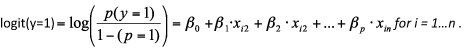
\includegraphics[scale=0.5]{mult.jpg} 
\linebreak
Source: https://www.statisticssolutions.com/mlr/
\end{center}

This model is appropriate because it results in something fairly comparable to the current PRS, where each crime is assigned points (i.e., coefficients) that add up to a total score. In our main model, we also constrained the crime variables to produce non-negative coefficients due to practical concerns of the impression that we were lowering one's PRS due to commission of certain crimes (which violates the retributive nature of the PRS and which we believed would make most criminal justice professionals and the general public uncomfortable). I have not forced this contraint on the current model, as it is my intention that this model not be used to replace the main PRS model, but as an added feature of the sentencing decision. For example, the current analysis may be used to flag high-felony-risk offenders. 

\section{Evaluaton Criteria and Results}

The current task is less concerned with predicting the actual outcome for each offender than in ranking offenders from lowest to highest risk of recidivism in order to construct a risk score for each offender. As a result, AUC will be a better metric by which to evaluate success than accuracy. The ROC curves on the next page show the outcome of my model with the associated AUCs for each class on the testing data. These AUCs are similar to the ones we have achieved in our main systems project research task, predicting any recidivism, so I believe this to be a good classifier given the available data. 

\pagebreak
\begin{center}
Figure 2: Model ROC and AUC Across 3 Outcome Levels
\end{center}
Felonies:
\begin{center}
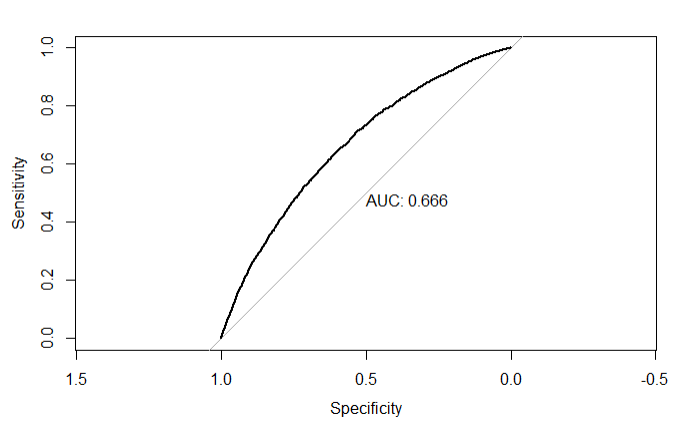
\includegraphics[scale=0.45]{felony.PNG}
\end{center}

Misdemeanors:
\begin{center}
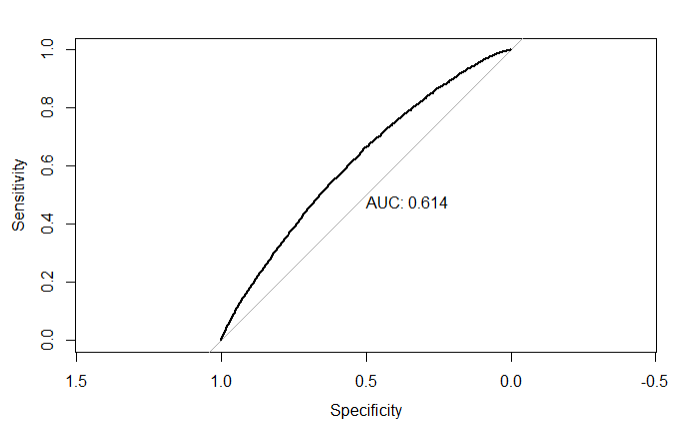
\includegraphics[scale=0.45]{misd.PNG}
\end{center}

No Recidivism:
\begin{center}
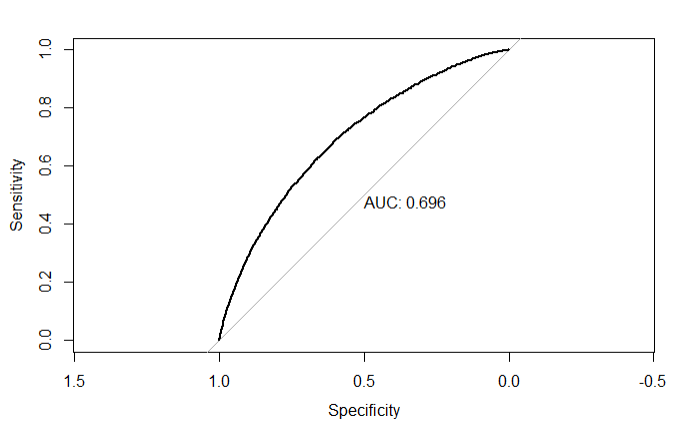
\includegraphics[scale=0.45]{norecid.PNG}
\end{center}
\pagebreak

The accuracy of my model overall was 0.49 (compared to a no information rate of 0.40). The balanced accuracy of each level was: 0.63 for no recidivism, 0.56 for misdemeanor recidivism, and 0.525 for felony recidivism. 

I then ran the same models with race, gender and age and obtain only slightly better results (AUCs of 0.682, 0.618 and 0.703 for the three classes, respectively). Since the inclusion of these variable is likely to raise red flags that might impede the implementation of such an approach, this confirmed the decision to leave these variables out of the model. 

Additionally, because the anticipated application of this model would be a flagging system for high-risk-felony offenders, a binary logistic model was also run to predict whether the offender would commit a felony after release, but had a slightly lower AUC as the current model (0.664).

To test for overfitting of the model, and whether I would need to perform lasso regularization to reduce the likelihood of overfitting, I observed the AUCs on the training data. The AUCs were almost identical to those on the testing data, so I do not believe overfitting is an issue in my model. 

\subsubsection{Model Fairness by Race}

One of the main criticisms of actuarial recidivism risk tools is that they tend to (unjustly) characterize more minority offenders as high risk than white offenders.\cite{propub} In some cases, the model may inherently "learn" things about race even though race is not used as an input to the model (and perhaps may even be more problematic when race is excluded from the model than when it is explicitly incorporated). 

When looking at actual recidivism outcome, our data does show that whites are less likely than other groups to be recidivate and be charged with a felony, and more likely than blacks to have no recidivism within 3 years. It is also worth noting that since we are measuring recidivism as being charged with a future offense and not as committing a future offense (which is unknowable), some of these differences may be due to disparities in policing (e.g., overpolicing, discrimination, etc.).  

\begin{center}
Table 2: Recidivism Type, Actual, by Race/Ethnicity (percent)
\begin{tabular}{ c c c c c }
  & White & Black & Hispanic & ALL \\ 
 No recidivism & 43.3 & 31.1 & 43.2 & 39.5 \\ 
 Misdemeanor & 42.0 & 39.0 & 35.7 & 40.5 \\ 
 Felony & 14.7 & 29.8 & 21.1 & 20.0\\ 
\end{tabular}
\end{center}

Overall, my model predicts a much lower incidence of felony recidivism than is present in the data (4.2 percent vs. 20 percent). Even more concerning is that while blacks are about 2 times as likely as whites to be rearrested for a felony in the observed outcomes, they are more than 11 times more likely to be predicted as likely felony recidivists by the model. A similar but less dramatic pattern is present for Hispanics versus Whites (1.4 times in reality vs. 6.8 times in the prediction). 

\pagebreak
\begin{center}
Table 3: Recidivism Type, Predicted, by Race/Ethnicity (percent)
\begin{tabular}{ c c c c c }
  & White & Black & Hispanic & ALL \\ 
 No recidivism & 45.0 & 31.4 & 48.7 & 41.0 \\ 
 Misdemeanor & 54.0 & 58.5 & 45.2 & 54.7 \\ 
 Felony & 0.9 & 10.1 & 6.1 & 4.2\\ 
\end{tabular}
\end{center}

This can also be seen by observing the predicted probabilities for white and black offenders in the data:

\begin{center}
Figure 3: Predicted Probability of Felony Recidivism, by Race/Ethnicity
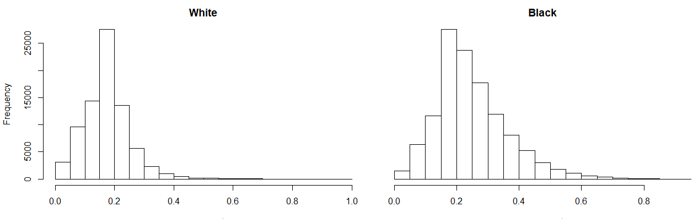
\includegraphics[scale=0.65]{histograms.PNG}
\end{center}

Some researchers have suggested that by including features like race in prediction models, we can actually make things more, not less, fair. However, an analysis of the alternative logistic regression model including age, gender and race shows an even more disparate impact in this regard. In that model, blacks are 67 times more likely to be predicted as high felony risk (17.6 percent vs. 0.3 percent) and Hispanics are about 15 times more likely (1.3 percent vs. 0.3 percent). This model predicts a higher overall level of felony recidivism (6.1 percent), but it does so while lowering the proportion predicted as such for whites and Hispanics and raising the levels for blacks. 

Another option is to build the model using race, but apply the model without any race information included. Running the model trained with demographic variables, but assigning every case to race = "Black", narrows but does not eliminate the disparity: 3.1 percent of whites, 17.6 percent of blacks and 12.3 percent of Hispanics are predicted to recidivate with felonies using this technique.

A final way to consider the fairness of this model is to look at its ROC curves across the three major racial groups. The AUCs for the felony class are higher for blacks (0.647) and Hispanics (0.673) than for whites (0.633), indicating that while minority groups might be more likely to be predicted in the felony class, the predicted probabilities that they are felony offenders are ranked slightly better within each racial group. 


\section{Conclusion}

Based on these results, it seems that this model could be incorporated into the sentencing decision in some way, but caution would need to be taken to ensure that it did not result in discriminatory outcomes. For example, the model could be used to flag people with high likelihood of felony recidivism by identifying offenders in the top quartile for predicted felony recidivism (corresponding to a predicted felony probability of 0.24 or higher, just above the mean predicted value of 0.2). However, because of the imbalance in predicted risks by race/ethnicity, this would lead to unfair application across race and ethnicity. In particular, it would assign 44 percent of black offenders, 31 percent of Hispanic offenders, and just 14 percent of white offenders as high risk of felony recidivism. 

Adjustments could be made to make the result of such a flagging mechanism less discriminatory by race. For example, one could flag the most risky individuals at a level equal to to the known felony recidivism rate in the population. For example, since 29.8 percent of blacks recidivate with felonies in reality, you could flag the riskiest 29.8 percent of blacks as high risk. This would correspond to assigning whites with predicted probabilities of 0.2405 or greater as high risk (n=11,513), blacks with predicted probabilities of 0.287 or greater as high risk (n=12,225), and Hispanics with predicted probabilities of 0.277 or greater as high risk (n=1,967).

\begin{thebibliography}{9}

\bibitem{code} 
The Pennsylvania Code, Chapter 303: Sentencing Guidelines,
\\\texttt{https://www.pacode.com/secure/data/204/chapter303/chap303toc.html}

\bibitem{review}
James, N. (2015) Risk and Needs Assessment in the Criminal Justice System. Congressional Research Service.
\\\texttt{https://fas.org/sgp/crs/misc/R44087.pdf}

\bibitem{borden} 
Borden, H. G. (1928) Factors for predicting parole success. J. Am. Inst. Crimnl Law Crim., 328–336.

\bibitem{burgess} 
Burgess, E. W. (1928) Factors determining success or failure on parole. Illinois Committee on Indeterminate‐Sentence Law and Parole, Springfield.

\bibitem{dawes} 
Dawes, R. M., Faust, D. and Meehl, P. E. (1989) Clinical versus actuarial judgment. Science, 243, 1668–1674.

\bibitem{grove_and_meehl} 
Grove, W. M. and Meehl, P. E. (1996) Comparative efficiency of informal (subjective, impressionistic) and formal (mechanical, algorithmic) prediction procedures: the clinical–statistical controversy. Psychol. Publ. Poly Law, 2, 293–323.

\bibitem{violence}
Prell, L, MJ Vitacco, & D Zavodny. (2016). Predicting violence and recidivism in a large sample of males on probation or parole. Int J Law Psychiatry 49(Pt A):107-113. \\\texttt{https://www.ncbi.nlm.nih.gov/pubmed/27686952}

\pagebreak
\bibitem{zeng}
Zeng, J., Ustun, B. and Rudin, C. (2016) Interpretable classification models for recidivism prediction. Journal of the Royal Statistical Society, 180(3), 689-722. 
\\\texttt{https://doi.org/10.1111/rssa.12227}

\bibitem{freak} 
Dubner, Stephen. (2011). Freakonomics Quorum: Why, During a Bad Economy, Does Crime Continue to Fall?,
\\\texttt{http://freakonomics.com/2011/06/08/freakonomics-quorum-why-during-a-bad-economy-does-crime-continue-to-fall/}

\bibitem{ucla} UCLA's Institute for Digital Research and Education. ORDINAL LOGISTIC REGRESSION: R DATA ANALYSIS EXAMPLES,
\\\texttt{https://stats.idre.ucla.edu/r/dae/ordinal-logistic-regression/}

\bibitem{propub}
Angwin, J., and Larson, J. (2016) Bias in Criminal Risk Scores Is Mathematically Inevitable, Researchers Say. ProPublica. 
\\\texttt{https://www.propublica.org/article/bias-in-criminal-risk-scores-is-mathematically-inevitable-researchers-say}

\end{thebibliography} 
\end{document}
